% -----------------------------*- LaTeX -*------------------------------
\documentclass[UTF8]{report}
% ------------------------------------------------------------------------
% Packages
% ------------------------------------------------------------------------
\usepackage{ctex} % 支持中文
\usepackage[body={7in, 9in},left=1in,right=1in]{geometry} % 改变页边距
\usepackage{amsmath} % AMS 的数学宏包
\usepackage{amsfonts} % AMS 的数学字体宏包
\usepackage{amssymb} % AMS 符号库
\usepackage{bm} % 数学公式中的黑斜体
\usepackage{amsthm} % AMS 的定理环境宏包
\usepackage{graphicx} % 插图
\usepackage{subfigure} % 插子图
\usepackage{nicefrac} % 好看的分数
\usepackage{mathrsfs} % mathscr font
\usepackage{caption} % caption
\usepackage{algorithm,algorithmicx} % 伪代码支持宏包
\usepackage[noend]{algpseudocode} % 伪代码
\usepackage{fancyhdr} % 设置页眉、页脚
\usepackage{adjustbox} % 图片尺寸自动调整
\usepackage{esint} % 积分符号
\usepackage{mathtools} % 数学宏包的重要补充
\usepackage{upgreek} % 数学环境的直立希腊字母
\usepackage{enumitem} % 使用enumitem宏包, 改变列表项的格式
\usepackage{color} % 支持彩色
\usepackage{extarrows} % 任意长度的箭头
\usepackage{tikz} % 绘图
\usepackage{forest} % 绘树
\usepackage{xcolor} % 颜色宏包
\usepackage{breqn} % 公式自动换行
\usepackage{fontsize} % 字体大小
\usepackage[framemethod=TikZ]{mdframed} % 给文字加框
\usepackage{fontspec} % 字体库
\usepackage{bigstrut} % 用于表格中的换行
\usepackage{multirow} % 表格中多行单元格合并
\usepackage{multicol} % 表格中多列单元格合并
\usepackage{longtable} % 长表格
\usepackage{rotating} % 旋转图形和表格      以上三者用于绘制三线表
\usepackage{booktabs} % 三线表宏包
\usepackage{scribe} % Scribe 模板
\usepackage{diagbox} % 表格斜线
\usepackage{listings} % 插入代码
\usepackage{verbatim} % 多行注释
\usepackage{ifplatform} % 检测编译平台
\usepackage{pifont} % 圆圈数字
\usetikzlibrary{shapes.geometric, arrows} % 引入流程图需要的库
\usetikzlibrary{automata} % 引入automata库
\usetikzlibrary{shapes,arrows,positioning,chains} % 引入positioning库
% ------------------------------------------------------------------------
% Macros
% ------------------------------------------------------------------------
%~~~~~~~~~~~~~~~
% Utility latin
%~~~~~~~~~~~~~~~
\newcommand{\ie}{\textit{i.e.}}
\newcommand{\eg}{\textit{e.g.}}
%~~~~~~~~~~~~~~~
% Environment shortcuts
%~~~~~~~~~~~~~~~
\newcommand{\balign}[1]{\ealign{\begin{align}#1\end{align}}}
\newcommand{\baligns}[1]{\ealigns{\begin{align*}#1\end{align*}}}
\newcommand{\bitemize}[1]{\eitemize{\begin{itemize}#1\end{itemize}}}
\newcommand{\benumerate}[1]{\eenumerate{\begin{enumerate}#1\end{enumerate}}}
%~~~~~~~~~~~~~~~
% Text with quads around it
%~~~~~~~~~~~~~~~
\newcommand{\qtext}[1]{\quad\text{#1}\quad}
%~~~~~~~~~~~~~~~
% Shorthand for math formatting
%~~~~~~~~~~~~~~~
\newcommand{\mbb}[1]{\mathbb{#1}}
\newcommand{\mbi}[1]{\boldsymbol{#1}} % Bold and italic (math bold italic)
\newcommand{\mbf}[1]{\mathbf{#1}}
\newcommand{\mc}[1]{\mathcal{#1}}
\newcommand{\mrm}[1]{\mathrm{#1}}
\newcommand{\tbf}[1]{\textbf{#1}}
\newcommand{\tsc}[1]{\textsc{#1}}
%\def\\langle {{\langle }}
%\def\\rangle {{\rangle }}
\newcommand{\sT}{\sf T}
\newcommand{\grad}{\nabla}
\newcommand{\Proj}{\Pi}
%~~~~~~~~~~~~~~~
% Common sets 定义数集符号
%~~~~~~~~~~~~~~~
\newcommand{\R}{\mathbb{R}}
\newcommand{\Z}{\mathbb{Z}}
\newcommand{\Q}{\mathbb{Q}}
\newcommand{\N}{\mathbb{N}}
\newcommand{\C}{\mathbb{C}}
\newcommand{\reals}{\mathbb{R}} % Real number symbol
\newcommand{\integers}{\mathbb{Z}} % Integer symbol
\newcommand{\rationals}{\mathbb{Q}} % Rational numbers
\newcommand{\naturals}{\mathbb{N}} % Natural numbers
\newcommand{\complex}{\mathbb{C}} % Complex numbers
%~~~~~~~~~~~~~~~
% Common functions
%~~~~~~~~~~~~~~~
\renewcommand{\exp}[1]{\operatorname{exp}\left(#1\right)} % Exponential
\newcommand{\indic}[1]{\mbb{I}\left(#1\right)} % Indicator function
\newcommand{\indicsub}[2]{\mbb{I}_{#2}\left(#1\right)} % Indicator function
\newcommand{\argmax}{\mathop\mathrm{arg\, max}} % Defining math symbols
\newcommand{\argmin}{\mathop\mathrm{arg\, min}}
\renewcommand{\arccos}{\mathop\mathrm{arccos}}
\newcommand{\dom}{\mathop\mathrm{dom}} % Domain
\newcommand{\range}{\mathop\mathrm{range}} % Range
\newcommand{\diag}{\mathop\mathrm{diag}}
\newcommand{\tr}{\mathop\mathrm{tr}}
\newcommand{\abs}{\mathop\mathrm{abs}}
\newcommand{\card}{\mathop\mathrm{card}}
\newcommand{\sign}{\mathop\mathrm{sign}}
\newcommand{\prox}{\mathrm{prox}} % prox
\newcommand{\rank}[1]{\mathrm{rank}(#1)}
\newcommand{\supp}[1]{\mathrm{supp}(#1)}
\newcommand{\norm}[1]{\lVert#1\rVert}
%~~~~~~~~~~~~~~~
% Common probability symbols
%~~~~~~~~~~~~~~~
\newcommand{\family}{\mathcal{P}} % probability family / statistical model
\newcommand{\iid}{\stackrel{\mathrm{iid}}{\sim}}
\newcommand{\ind}{\stackrel{\mathrm{ind}}{\sim}}
\newcommand{\E}{\mathbb{E}} % Expectation symbol
\newcommand{\Earg}[1]{\E\left[#1\right]}
\newcommand{\Esubarg}[2]{\E_{#1}\left[#2\right]}
\renewcommand{\P}{\mathbb{P}} % Probability symbol
\newcommand{\Parg}[1]{\P\left(#1\right)}
\newcommand{\Psubarg}[2]{\P_{#1}\left[#2\right]}
%\newcommand{\Cov}{\mrm{Cov}} % Covariance symbol
%\newcommand{\Covarg}[1]{\Cov\left[#1\right]}
%\newcommand{\Covsubarg}[2]{\Cov_{#1}\left[#2\right]}
%\newcommand{\model}{\mathcal{P}} % probability family / statistical model
%~~~~~~~~~~~~~~~
% Distributions
%~~~~~~~~~~~~~~~
%\newcommand{\Gsn}{\mathcal{N}}
%\newcommand{\Ber}{\textnormal{Ber}}
%\newcommand{\Bin}{\textnormal{Bin}}
%\newcommand{\Unif}{\textnormal{Unif}}
%\newcommand{\Mult}{\textnormal{Mult}}
%\newcommand{\NegMult}{\textnormal{NegMult}}
%\newcommand{\Dir}{\textnormal{Dir}}
%\newcommand{\Bet}{\textnormal{Beta}}
%\newcommand{\Gam}{\textnormal{Gamma}}
%\newcommand{\Poi}{\textnormal{Poi}}
%\newcommand{\HypGeo}{\textnormal{HypGeo}}
%\newcommand{\GEM}{\textnormal{GEM}}
%\newcommand{\BP}{\textnormal{BP}}
%\newcommand{\DP}{\textnormal{DP}}
%\newcommand{\BeP}{\textnormal{BeP}}
%\newcommand{\Exp}{\textnormal{Exp}}
%~~~~~~~~~~~~~~~
% Theorem-like environments
%~~~~~~~~~~~~~~~
%\theoremstyle{definition}
%\newtheorem{definition}{Definition}
%\newtheorem{example}{Example}
%\newtheorem{problem}{Problem}
%\newtheorem{lemma}{Lemma}
%~~~~~~~~~~~~~~~
% 组合数学的模板和作业里用到的一些宏包和自定义命令
%~~~~~~~~~~~~~~~
\renewcommand{\emph}[1]{\begin{kaishu}#1\end{kaishu}}
\newcommand{\falfac}[1]{^{\underline{#1}}}
\newcommand{\binomfrac}[2]{\frac{#1^{\underline{#2}}}{#2!}}
\newcommand{\ceil}[1]{\left\lceil #1 \right\rceil}
\newcommand{\floor}[1]{\left\lfloor #1 \right\rfloor}
\newcommand{\suminfty}[2]{\sum_{#1=#2}^{\infty}}
\newcommand{\suminftyk}[0]{\sum_{k=0}^{\infty}}
\newcommand{\sumint}[3]{\sum_{#1=#2}^{#3}}
\newcommand{\sumintk}[2]{\sum_{k=#1}^{#2}}
\newcommand{\suminti}[2]{\sum_{i=#1}^{#2}}
%~~~~~~~~~~~~~~~
% 定义新命令
%~~~~~~~~~~~~~~~
\newcommand*{\unit}[1]{\mathop{}\!\mathrm{#1}}
\newcommand*{\dif}{\mathop{}\!\mathrm{d}}%微分算子 d
\newcommand*{\pdif}{\mathop{}\!\partial}%偏微分算子
\newcommand*{\cdif}{\mathop{}\!\nabla}%协变导数、nabla 算子
\newcommand*{\laplace}{\mathop{}\!\Delta}%laplace 算子
\newcommand*{\deri}[1]{\mathrm{d} #1}
\newcommand*{\deriv}[2]{\frac{\mathrm{d} #1}{\mathrm{d} {#2}}}
\newcommand*{\derivh}[3]{\frac{\mathrm{d}^{#1} #2}{\mathrm{d} {#3^{#1}}}}
\newcommand*{\pderiv}[2]{\frac{\partial #1}{\partial {#2}}}
\newcommand*{\pderivh}[3]{\frac{\partial^{#1} #2}{\partial {#3^{#1}}}}
\newcommand*{\dderiv}[2]{\dfrac{\mathrm{d} #1}{\mathrm{d} {#2}}}
\newcommand*{\dderivh}[3]{\dfrac{\mathrm{d}^{#1} #2}{\mathrm{d} {#3^{#1}}}}
\newcommand*{\dpderiv}[2]{\dfrac{\partial #1}{\partial {#2}}}
\newcommand*{\dpderivh}[3]{\dfrac{\partial^{#1} #2}{\partial {#3^{#1}}}}
\newcommand{\me}[1]{\mathrm{e}^{#1}}%e 指数
\newcommand{\mi}{\mathrm{i}}%虚数单位
%\newcommand{\mc}{\mathrm{c}}%光速 定义与mathcal冲突
\newcommand{\red}[1]{\textcolor{red}{#1}}
\newcommand{\blue}[1]{\textcolor{blue}{#1}}
%\newcommand{\Rome}[1]{\setcounter{rome}{#1}\Roman{rome}}
%~~~~~~~~~~~~~~~
% 公式环境中箭头符号的简写
%~~~~~~~~~~~~~~~
\newcommand{\ra}{\rightarrow}
\newcommand{\Ra}{\Rightarrow}
\newcommand{\la}{\leftarrow}
\newcommand{\La}{\Leftarrow}
\newcommand{\lra}{\leftrightarrow}
\newcommand{\Lra}{\Leftrightarrow}
\newcommand{\lgla}{\longleftarrow}
\newcommand{\Lgla}{\Longleftarrow}
\newcommand{\lgra}{\longrightarrow}
\newcommand{\Lgra}{\Longrightarrow}
\newcommand{\lglra}{\longleftrightarrow}
\newcommand{\Lglra}{\Longleftrightarrow}
%~~~~~~~~~~~~~~~
% 一些数学的环境设置
%~~~~~~~~~~~~~~~
%\newcounter{counter_exm}\setcounter{counter_exm}{1}
%\newcounter{counter_prb}\setcounter{counter_prb}{1}
%\newcounter{counter_thm}\setcounter{counter_thm}{1}
%\newcounter{counter_lma}\setcounter{counter_lma}{1}
%\newcounter{counter_dft}\setcounter{counter_dft}{1}
%\newcounter{counter_clm}\setcounter{counter_clm}{1}
%\newcounter{counter_cly}\setcounter{counter_cly}{1}
\newtheorem{theorem}{{\hskip 1.7em \bf 定理}}
\newtheorem{lemma}[theorem]{\hskip 1.7em 引理}
\newtheorem{proposition}[theorem]{\hskip 1.7em 命题}
\newtheorem{claim}[theorem]{\hskip 1.7em 断言}
\newtheorem{corollary}[theorem]{\hskip 1.7em 推论}
% \newcommand{\problem}[1]{{\setlength{\parskip}{10pt}\noindent \bf{#1}}}
\newenvironment{solution}{{\noindent \bf 解 \quad}}{}
\newenvironment{remark}{{\noindent \bf 注 \quad}}{}
\newenvironment{definition}{{\noindent \bf 定义 \quad}}{}
\renewenvironment{proof}{{\setlength{\parskip}{7pt}\noindent\hskip 2em \bf 证明 \quad}}{\hfill$\qed$\par}
\newenvironment{example}{{\noindent\bf 例 \quad}}{\hfill$\qed$\par}
%\newenvironment{concept}[1]{{\bf #1\quad} \begin{kaishu}} {\end{kaishu}\par}
%~~~~~~~~~~~~~~~
% 本.tex文档中特殊定义命令
%~~~~~~~~~~~~~~~
\newcommand{\lno}[1]{\overline{#1}}
\newcommand{\NP}{\mathrm{NP}}
\newcommand{\coNP}{\mathrm{coNP}}
% \newcommand{\ISO}{\mathrm{ISO}}
\newcommand{\SAT}{\mathrm{SAT}}
\newcommand{\USAT}{\mathrm{USAT}}
% \newcommand{\threeSAT}{\mathrm{3\text{-}SAT}}
\renewcommand{\P}{\mathrm{P}}
% \mathchardef\mhyphen="2D
% \newcommand{\CNF}{\mathrm{CNF}}
% \newcommand{\DNF}{\mathrm{DNF}}
% \newcommand{\SetSp}{\mathrm{SET\text{-}SPLITTING}}
% \newcommand{\PUZZLE}{\mathrm{PUZZLE}}
% \newcommand{\SPATH}{\mathrm{SPATH}}
% \newcommand{\LPATH}{\mathrm{LPATH}}
% \newcommand{\UHAMPATH}{\mathrm{UHAMPATH}}
\newcommand{\SPACE}{\mathrm{SPACE}}
\newcommand{\NSPACE}{\mathrm{NSPACE}}
\newcommand{\PSPACE}{\mathrm{PSPACE}}
\newcommand{\NPSPACE}{\mathrm{NPSPACE}}
\newcommand{\DFA}{\mathrm{DFA}}
\newcommand{\NFA}{\mathrm{NFA}}
\newcommand{\TQBF}{\mathrm{TQBF}}
% \newcommand{\L}{\mathrm{L}}
\renewcommand{\O}{\mathrm{O}}
\newcommand{\NL}{\mathrm{NL}}
\newcommand{\coNL}{\mathrm{coNL}}
\newcommand{\LADDER}{\mathrm{LADDER_{DFA}}}
\newcommand{\hd}{\mathrm{\text{-}hard}}
\newcommand{\ADD}{\mathrm{ADD}}
\newcommand{\STCN}{\mathrm{STRONGLY\text{-}CONNECTED}}
\newcommand{\PATH}{\mathrm{PATH}}
\newcommand{\A}{\mathrm{A}}
%使用align环境公式换页
\allowdisplaybreaks[4]

\definecolor{dkgreen}{rgb}{0,0.6,0}
\definecolor{gray}{rgb}{0.5,0.5,0.5}
\definecolor{mauve}{rgb}{0.58,0,0.82}
\lstset{
  frame=tb,
  aboveskip=3mm,
  belowskip=3mm,
  showstringspaces=false,
  columns=flexible,
  framerule=1pt,
  rulecolor=\color{gray!35},
  backgroundcolor=\color{gray!5},
  basicstyle={\small\ttfamily},
  numbers=none,
  numberstyle=\tiny\color{gray},
  keywordstyle=\color{blue},
  commentstyle=\color{dkgreen},
  stringstyle=\color{mauve},
  breaklines=true,
  breakatwhitespace=true,
  tabsize=3,
}

\tikzstyle{startstop} = [rectangle, rounded corners, minimum width=3cm, minimum height=1cm,text centered, draw=black, fill=red!30]
\tikzstyle{process} = [rectangle, minimum width=3cm, minimum height=1cm, text centered, draw=black, fill=orange!30]
\tikzstyle{decision} = [diamond, minimum width=3cm, minimum height=1cm, text centered, draw=black, fill=green!30]
\tikzstyle{arrow} = [thick,->,>=stealth]

\ifwindows
    \setmainfont{Times New Roman}
    \setsansfont{Times New Roman}
    \setmonofont{Consolas}
    \setCJKmainfont{SimHei}
    \setCJKsansfont{SimSun}
    \setCJKmonofont{FangSong}
\fi

\ifmacosx
    \setmainfont{Times New Roman}
    \setsansfont{Times New Roman}
    \setmonofont{Menlo}
    \setCJKmainfont{STHeiti}
    \setCJKsansfont{STSong}
    \setCJKmonofont{STFangsong}
\fi

\punctstyle{kaiming}

\begin{document}

\pagestyle{fancy}

\reporttype{Report}                 % required
\course{Lab of Computer Network} 				% optional
\coursetitle{IP\_Lookup}	    % optional
\semester{Fall 2024}			    % optional
\lecturer{Wu Qinghua}			% optional
\scribe{2022K8009929010 Zhang Jiawei}			% required
\lecturenumber{10}				% required (must be a number)
\lecturedate{Novmeber 12}			% required (omit year)
\maketitle

\section{实验内容}

\begin{enumerate}
    \item 实现最基本的前缀树查找
    \item 调研并实现某种优化的IP前缀查找方案
    \item 对比基本前缀树和所实现IP前缀查找的性能(内存开销、平均单次查找时间)
\end{enumerate}

\section{实验过程}

\subsection{基本前缀树查找}

基本前缀树查找包括构建前缀树和查找前缀树两个部分。基本前缀树节点的数据结构已经在头文件中给出,我们只需要完成构建和查找的函数即可。

前缀树的构建基于数据库。我读取数据库中每一行的IP地址、前缀长度和端口号,然后将其插入到前缀树中。我用一个32位的数组来存储读取到的IP地址的二进制表示,从高位到低位,每次读取一位,如果该位为1,则向右子树移动,若右子树为空则申请空间构建右子节点,否则向左子树移动,若左子树为空则申请空间构建左子节点。当读取完前缀长度对应的IP地址后,将端口号存储在到达的节点中,且设置节点类型为匹配节点。代码如下:

\begin{lstlisting}[language=C]
    // Constructing an basic trie-tree to lookup according to `forward_file`
    void create_tree(const char* forward_file)
    {
        // fprintf(stderr,"TODO:%s",__func__);
        root = (node_t *)malloc(sizeof(node_t));
        root->type = I_NODE;
        root->lchild = NULL;
        root->rchild = NULL;
        size += sizeof(node_t);
    
        FILE *fp = fopen(forward_file, "r");
        if (fp == NULL) {
            fprintf(stderr, "Error: cannot open file %s\n", forward_file);
            exit(1);
        }
    
        char line[100];
        while (fgets(line, 100, fp) != NULL) {
            char ip_str[15];
            uint32_t port, prefix;
            sscanf(line, "%s %u %u", ip_str, &prefix, &port);
            int ip_dec[4];
            sscanf(ip_str, "%d.%d.%d.%d", &ip_dec[0], &ip_dec[1], &ip_dec[2], &ip_dec[3]);
            
            uint32_t ip_bin[32];
            for (int i = 0; i < 4; i++) 
                for (int j = 7; j >= 0; j--) 
                    ip_bin[i * 8 + 7 - j] = (ip_dec[i] >> j) & 1;
    
            node_t *cur = root;
            for (int i = 0; i < prefix; i++) {
                if (ip_bin[i] == LEFT) {
                    if (cur->lchild == NULL) {
                        cur->lchild = (node_t *)malloc(sizeof(node_t));
                        cur->lchild->type = I_NODE;
                        cur->lchild->lchild = NULL;
                        cur->lchild->rchild = NULL;
                        size += sizeof(node_t);
                    }
                    cur = cur->lchild;
                }
                else if (ip_bin[i] == RIGHT) {
                    if (cur->rchild == NULL) {
                        cur->rchild = (node_t *)malloc(sizeof(node_t));
                        cur->rchild->type = I_NODE;
                        cur->rchild->lchild = NULL;
                        cur->rchild->rchild = NULL;
                        size += sizeof(node_t);
                    }
                    cur = cur->rchild;
                }
                else {
                    fprintf(stderr, "Error: invalid ip\n");
                    exit(1);
                }
            }
    
            cur->type = M_NODE;
            cur->port = port;
        }
    
        fclose(fp);
        return;
    }
\end{lstlisting}

查找前缀树的过程是根据输入的IP地址,从根节点开始,根据IP地址的每一位向下查找,直到无法继续向下查找为止。查找的过程中,如果遇到匹配节点,则更新查找到的端口号。这样的操作是满足最长前缀匹配的,代码如下:

\begin{lstlisting}[language=C]
    // Look up the ports of ip in file `ip_to_lookup.txt` using the basic tree, input is read from `read_test_data` func 
    uint32_t *lookup_tree(uint32_t* ip_vec)
    {
        // fprintf(stderr,"TODO:%s",__func__);
        uint32_t *port_vec = (uint32_t *)malloc(sizeof(uint32_t) * TEST_SIZE);
        for (int i = 0; i < TEST_SIZE; i++)
        {
            uint32_t ip_bin[32];
            for (int j = 0; j < 32; j++) 
                ip_bin[j] = (ip_vec[i] >> j) & 1;
                    
            node_t *cur = root;
            port_vec[i] = -1;
            int idx = 31;
            while (idx >= 0) {
                if (cur->type == M_NODE) 
                    port_vec[i] = cur->port;
                
                if (ip_bin[idx] == LEFT) {
                    if (cur->lchild == NULL) 
                        break;
                    cur = cur->lchild;
                }
                else if (ip_bin[idx] == RIGHT) {
                    if (cur->rchild == NULL) 
                        break;
                    cur = cur->rchild;
                }
                else {
                    fprintf(stderr, "Error: invalid ip\n");
                    exit(1);
                }
                idx--;
            }
        }
    
        return port_vec;
    }    
\end{lstlisting}

\subsection{优化前缀树查找}

这里我采取的思路是,先根据IP地址的前16位进行分类,如果直接映射到对应的前16位,则继续以2位为索引查找后16位,否则直接返回。这样的操作可以减少查找的次数,提高查找的效率。但是,前缀长度可能不是2的倍数,所以我多增加了一个域表示匹配节点的前缀是奇数还是偶数。节点的数据结构如下:

\begin{lstlisting}[language=C]
    typedef struct node_advance{
        bool type; //I_NODE or M_NODE
        uint32_t port;
        int prefix_diff; // 0 for even, 1 for odd
        struct node_advance* child[4];
    }node_advance_t;
\end{lstlisting}    

构建前缀树时需要考虑的内容比较多。如果前缀长度小于16,则会映射到多个表项中,需要一一遍历这些表项根节点进行更新,更新条件是根节点为中间节点或者前缀长度不大于新节点的前缀长度。前缀长度不小于16时,就需要对相应根节点的子节点进行插入操作,根据IP的每两位进行索引,如果子节点为空则申请空间构建子节点,继续向下插入。此时若遇到前缀长度为奇数则将前缀差设置为1,然后更新节点类型为匹配节点,端口号存储在该节点中。代码如下:

\begin{lstlisting}[language=C]
    // Constructing an advanced trie-tree to lookup according to `forward_file`
    void create_tree_advance(const char* forward_file)
    {
        // fprintf(stderr,"TODO:%s",__func__);
        notmatch = (node_advance_t *)malloc(sizeof(node_advance_t));
        notmatch->port = -1;
        for (int i = 0; i < MAP_NUM; i++){
            triemap[i] = (node_advance_t *)malloc(sizeof(node_advance_t));
            triemap[i]->port = 0;
            triemap[i]->prefix_diff = 0;
            triemap[i]->type = I_NODE;
            for (int j = 0; j < 4; j++)
                triemap[i]->child[j] = NULL;
            size_advance += sizeof(node_advance_t);
        }
    
        FILE *fp = fopen(forward_file, "r");
        if (fp == NULL) {
            fprintf(stderr, "Error: cannot open file %s\n", forward_file);
            exit(1);
        }
    
        char line[100];
        while (fgets(line, 100, fp) != NULL) {
            char ip_str[15];
            uint32_t port, prefix;
            sscanf(line, "%s %u %u", ip_str, &prefix, &port);
            int ip_dec[4];
            sscanf(ip_str, "%d.%d.%d.%d", &ip_dec[0], &ip_dec[1], &ip_dec[2], &ip_dec[3]);
            
            uint32_t ip_bin = 0;
            for (int i = 0; i < 4; i++) 
                ip_bin |= (ip_dec[i] << (3 - i) * 8);
            
            if (prefix >= MAP_SHIFT){
                node_advance_t *root = triemap[(ip_bin & 0xffff0000) >> MAP_SHIFT];
                node_advance_t *cur = root, *next = NULL;
                int offset, cur_bit, cur_prefix;
    
                for (cur_prefix = 32-MAP_SHIFT; cur_prefix < prefix-1; cur_prefix+=2){
                    offset = 30 - cur_prefix;
                    cur_bit = (ip_bin >> offset) & 0x3;
                    next = cur->child[cur_bit];
                    if (next == NULL){
                        next = (node_advance_t *)malloc(sizeof(node_advance_t));
                        next->port = 0;
                        next->prefix_diff = 0;
                        next->type = I_NODE;
                        for (int j = 0; j < 4; j++)
                            next->child[j] = NULL;
                        cur->child[cur_bit] = next;
                        size_advance += sizeof(node_advance_t);
                    }
                    cur = next;
                }
    
                if (cur_prefix == prefix - 1){
                    offset = 30 - cur_prefix;
                    cur_bit = (ip_bin >> offset) & 0x3;
                    int start_bit = cur_bit & 0x2;
                    for (int i = 0; i < 2; i++){
                        next = cur->child[start_bit + i];
                        if (next == NULL){
                            next = (node_advance_t *)malloc(sizeof(node_advance_t));
                            next->port = port;
                            next->prefix_diff = 1;
                            next->type = M_NODE;
                            for (int j = 0; j < 4; j++)
                                next->child[j] = NULL;
                            cur->child[start_bit + i] = next;
                            size_advance += sizeof(node_advance_t);
                        }
                    }
                }
                else{
                    cur->port = port;
                    cur->type = M_NODE;
                }
            }
            else{
                uint32_t mask = 0xffffffff << (32 - prefix);
                uint32_t start = (ip_bin & mask) >> MAP_SHIFT;
                uint32_t end = start + (1 << (MAP_SHIFT - prefix));
                for (int i = start; i < end; i++){
                    if (triemap[i]->type == I_NODE || triemap[i]->prefix_diff >= 16 - prefix){
                        triemap[i]->port = port;
                        triemap[i]->type = M_NODE;
                        triemap[i]->prefix_diff = 16 - prefix;
                    }
                }
            }
        }   
            
        fclose(fp);
        return;
    }    
\end{lstlisting}

查找前缀树的过程比较类似,只是在查找的过程中,我设计一个match节点来存储匹配到的节点内容,需要根据IP的前16位找到对应的根节点,然后根据IP的后16位进行查找。查找的过程中,如果遇到匹配节点,则更新match节点的状态。代码如下:

\begin{lstlisting}[language=C]
    // Look up the ports of ip in file `ip_to_lookup.txt` using the advanced tree input is read from `read_test_data` func 
    uint32_t *lookup_tree_advance(uint32_t* ip_vec)
    {
        // fprintf(stderr,"TODO:%s",__func__);
        uint32_t *port_vec = (uint32_t *)malloc(sizeof(uint32_t) * TEST_SIZE);
    
        for (int i = 0; i < TEST_SIZE; i++)
        {
            uint32_t ip = ip_vec[i];
            node_advance_t *cur = triemap[ip >> MAP_SHIFT];
            node_advance_t *match = notmatch;
    
            uint32_t cur_bit;
            int cur_prefix = 32 - MAP_SHIFT;
    
            if (cur->prefix_diff > 0){
                if (cur->type == M_NODE)
                    match = cur;
                cur_bit = (ip >> 14) & 0x3;
                cur = cur->child[cur_bit];
                cur_prefix += 2;
            }
    
            while (cur != NULL){
                if (cur->type == M_NODE)
                    match = cur;
                int offset = 30 - cur_prefix;
                cur_bit = (ip >> offset) & 0x3;
                cur = cur->child[cur_bit];
                cur_prefix += 2;
            }
    
            port_vec[i] = match->port;
        }   
            
        return port_vec;
    }    
\end{lstlisting}

\section{实验结果}

运行程序,得到的结果如下图所示:

\begin{figure}[H]
    \centering
    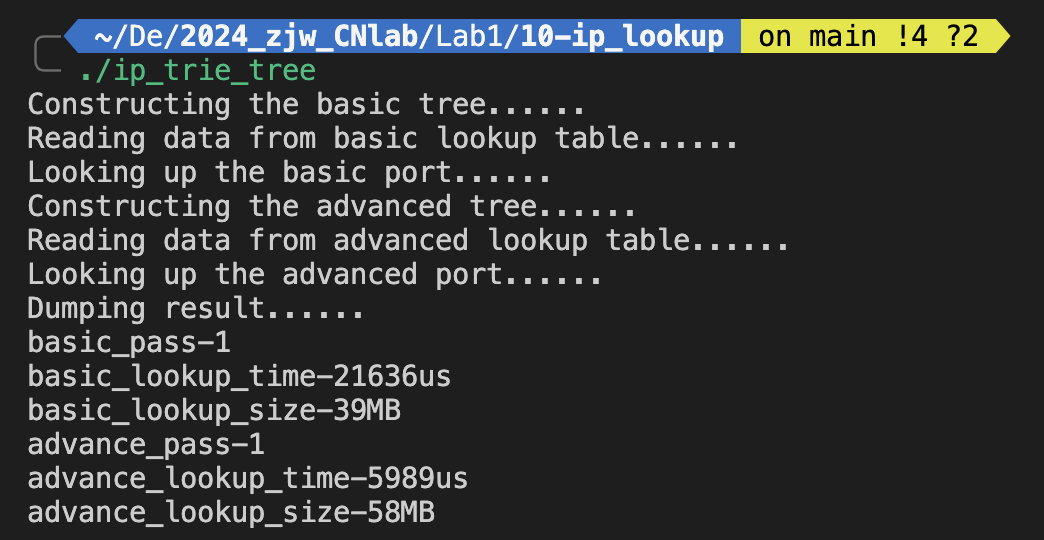
\includegraphics[width=0.7\textwidth]{result.png}
    \caption{实验结果}
\end{figure}

可以看出,在查找时间方面,优化前缀树查找的时间大概只有基本前缀树查找的1/4,这是因为优化前缀树查找的次数更少,查找效率更高。但是在内存方面,优化前缀树查找的内存开销大概是基本前缀树查找的1.5倍,这是因为优化前缀树查找的节点数据结构更复杂,需要更多的内存空间,这也是查找效率提高的代价。

\section{实验总结}

本次实验主要是实现了基本前缀树查找和优化前缀树查找,通过对比两者的性能,可以看出优化前缀树查找的效率更高,但是内存开销也更大。这是一个典型的时间和空间的权衡问题,需要根据实际情况选择合适的方案。
\end{document}